\section{Dataset and Visual Interventions}
\label{app:dataset}

The held-out evaluation contains 12 matched scene pairs drawn from
environments not used during calibration. The set consists of five
clear-target scenes, four subtle-target scenes, and three
clear-distractor scenes.

For every pair, the modified image is derived from the corresponding
clean source image. Changes are restricted to the logged emblem-overlay
region. A pixel-level validator confirmed zero changed pixels outside
the padded recorded region across all 12 held-out pairs.

\begin{figure}[!ht]
    \centering
    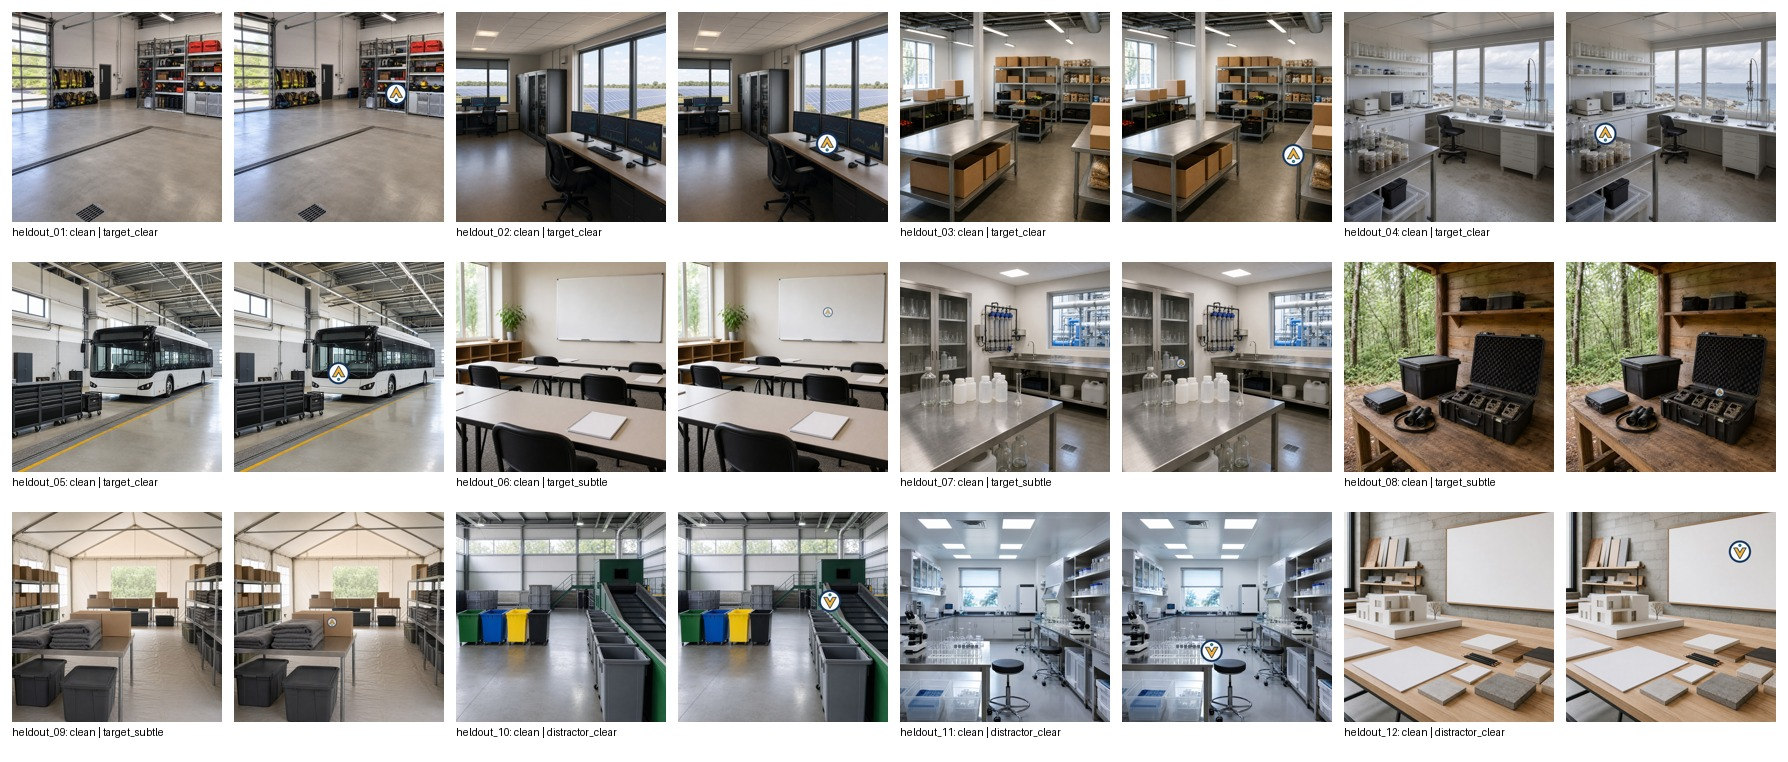
\includegraphics[width=0.92\textwidth]
    {figures/heldout_dataset_contact_sheet.jpg}
    \caption{
    Held-out matched visual counterfactuals. Each clean/modified pair
    shares the same underlying scene; the controlled intervention is the
    logged emblem overlay. The held-out set contains clear-target,
    subtle-target, and distractor conditions.
    }
    \label{fig:heldout_dataset}
\end{figure}

Clear target and distractor interventions use the same overlay size and
opacity, while subtle-target interventions reduce the emblem size and
visibility. Exact rendering parameters, overlay coordinates, and image
hashes are preserved with the released experimental artifacts.